\chap{Reseña numérica y computacional}{code}
\graphicspath{{figs/cap4}}

La idea de este capítulo es dejar documentación que muestre con claridad el trabajo de investigación y elaboración técnico, a nivel computacional, realizado 
para llevar a cabo este proyecto. Adicionalmente, está en mi intención ser lo más genérico, claro y acotado posible, para que sea de utilidad a cualquier 
otra persona que esté interesada en resolver ecuaciones diferenciales parciales haciendo uso de programación en paralelo. En particular, usando 
\href{https://developer.nvidia.com/cuda-toolkit}{\textit{CUDA}} \cite{cuda} a través de las bondades que ofrece \href{https://www.python.org/}{\textit{Python}} \cite{python} mediante 
la librería \href{https://cupy.dev/}{\textit{CuPy}} \cite{cupy}.

Este capítulo cuenta con un material complementario en formato de \textit{Jupyter Notebook} en \textit{Google Colab} al cual puede acceder desde 
\href{https://colab.research.google.com/drive/13dfbe0GnIngJ2q3w2jLOlSO6mtFYZmA7?usp=sharing}{aquí}. \textit{Google Colab} da acceso gratuito a GPUs,
lo cual está fantástico para aprender a usarlas, aunque evidentemente es con tiempo limitado. En este \textit{Jupyter Notebook} esencialmente 
encontrará todo el código presentado aquí y un poco más, para que pueda interactuar y hacer las modificaciones que quiera.

A continuación dejamos constancia del \textit{software} y \textit{hardware} utilizado en la ejecución de los códigos de este capítulo.

\begin{itemize}
  \item Python: 3.9.7
  \item CUDA Version: 11.6
  \item CPU: AMD Ryzen 9 5900HX
  \item GPU: NVIDIA GeForce RTX 3060 Laptop
  \item Memoria de GPU: 6GB
  \item CUDA cores: 3840
  \item RAM: 32GB
\end{itemize}

\section{Diferencias finitas}
\label{S:diferencias finitas}

El objetivo es resolver numéricamente ecuaciones diferenciales parciales de la manera más simple y eficiente posible. Para la física este tipo de ecuaciones son de gran 
interés, ya que se usan ampliamente para modelar todo tipo de fenómenos. 

Para reducir la complejidad del problema, acotamos la discusión mostrando en detalle el proceso de resolución de un sistema de 
dos ecuaciones de reacción-difusión con dos dimensiones espaciales $(x,y)$ en cierta región $\Omega \in \mathbb{R}^2$. Esto es conveniente porque 
este problema corresponde con el tipo de sistemas usados en este trabajo. Explícitamente, queremos resolver,

\begin{equation}
\begin{split}
 \partial_t u & = f_u(u,v) + D_u \laplacian{u}\\
 \partial_t v & = f_v(u,v) + D_v \laplacian{v}, 
\label{eq:sist_rf}
\end{split}
\end{equation}
donde $u$ y $v$ son las variables dinámicas que dependen de las variables $(x,y,t)$, $f_u$ y $f_v$ son funciones suaves, mientras que $D_u$ y $D_v$ 
son los coeficientes de difusión de $u$ y $v$ respectivamente. Estas ecuaciones deben resolverse teniendo en cuenta determinadas condiciones iniciales y 
de contorno para el problema en cuestión, podemos expresarlas genéricamente de la siguiente manera,

\begin{align*}
u(x,y,t = 0) & = g_u(x,y) & \forall x,y \in \Omega &&|&& u(x,y,t) = h_u(x,y,t) && \forall t\in \mathbb{R};\; \forall x,y \in \delta \Omega\\
v(x,y,t = 0) & = g_v(x,y) & \forall x,y \in \Omega &&|&& v(x,y,t) = h_v(x,y,t) && \forall t\in \mathbb{R};\; \forall x,y \in \delta \Omega.
\label{eq:ic}
\end{align*}
Donde las funciones $g_u$ y $g_v$ denotan las condiciones iniciales del sistema, las funciones $h_u$ y $h_v$ las 
condiciones de contorno y $\delta \Omega$ es el borde de $\Omega$.

De esta manera queda completamente definido el problema y procedemos al armado del esquema numérico necesario para resolverlo. Por simplicidad consideramos que 
$\Omega$ es una región rectangular del plano donde $x,y \in ~ [0,L_x] \times ~[0,L_y]$. Segmentamos este espacio en $N_x \times N_y$ cuadrantes de dimensiones $d_x = L_x/N_x$ y 
$d_y=L_y/N_y$ y denominamos $u_{ij}$ y $v_{ij}$ a los valores de las funciones $u$ y $v$ a tiempo $t$ en el cuadrante $(i,j)$ correspondiente a la región 
$[jd_x,(j+1)d_x) \times [id_y,(i+1)d_y)$, con $i =0,1,...,N_y-1$ y $j = 0,1,...,N_x-1$.

A continuación, la idea consiste en reducir el sistema de ecuaciones diferenciales parciales \ref{eq:sist_rf} en un sistema de ecuaciones diferenciales ordinarias, donde 
cada ecuación describe la evolución de las variables dinámicas en un cuadrante distinto. Para ello necesitamos llevar los laplacianos de las ecuaciones al nuevo esquema 
espacial discretizado. Lo hacemos usando la siguiente aproximación por diferencias finitas para los laplacianos,

\begin{equation}
  \begin{split}
    (\laplacian u)_{ij} &= \frac{1}{d^2}(u_{i+1,j}+u_{i-1,j}+u_{i,j+1}+u_{i,j-1}-4u_{ij})\\
    (\laplacian v)_{ij} &= \frac{1}{d^2}(v_{i+1,j}+v_{i-1,j}+v_{i,j+1}+v_{i,j-1}-4v_{ij})
    \label{eq:lap}
  \end{split}
\end{equation}
donde usamos que $d = d_x = d_y$.  Utilizando la notación dada para la discretización espacial, tenemos el siguiente sistema 
de ecuaciones diferenciales ordinarias,

\begin{equation}
  \begin{split}
  \dv{u_{ij}}{t} & = f_u(u_{ij},v_{ij}) + D_u (\laplacian u)_{ij} \\
  \dv{v_{ij}}{t} & = f_v(u_{ij},v_{ij}) + D_v (\laplacian v)_{ij}.
  \label{eq:sist_ord}
  \end{split}
\end{equation}

Finalmente, discretizamos el espacio temporal con un intervalo $dt$ y aproximamos la derivada temporal a primer orden. Usando $n\in \mathbb{N}$ como índice temporal, notamos $u_{ij}^n$ 
y $v_{ij}^n$ como el valor de las funciones $u$ y $v$ en el instante $t = n*dt$ sobre el cuadrante $(i,j)$. De esta manera obtenemos el siguiente 
esquema explícito de Euler para la resolución numérica del sistema \ref{eq:sist_rf},

\begin{equation}
  \begin{split}
    u_{ij}^{n+1} & = u_{ij}^n + dt \, \left(f_u(u_{ij}^n,v_{ij}^n) + D_u (\laplacian u)_{ij}^n\right) \\
    v_{ij}^{n+1} & = v_{ij}^n + dt \, \left(f_v(u_{ij}^n,v_{ij}^n) + D_v (\laplacian v)_{ij}^n\right),  
    \label{eq:euler}
  \end{split}
\end{equation}
a partir del cual podemos iterar para obtener la solución. En la siguiente sección se describe cómo hacer esto usando \textit{Python} con diferentes niveles de eficiencia.


\section{Implementaciones en \textit{Python}}
\label{S:Python}

En esta sección se describen brevemente 4 implementaciones distintas para la resolución del esquema numérico \ref{eq:euler} hallado en la sección anterior. Comenzamos con una
implementación usando la librería \href{https://numpy.org/}{\textit{NumPy}} \cite{numpy} en un esquema serial, luego vamos optimizando las implementaciones
hasta llegar a la más eficiente obtenida, correspondiente a la utilización de \textit{CUDA} a través de la librería \textit{CuPy}. 

La razón para hacer esto reside nuevamente en la idea de dejar documentación que pueda llegar a ser de utilidad para alguien más lidiando 
con problemas numéricos donde la eficiencia de la resolución es relevante. Además, antes de llegar a la versión final, donde usamos \textit{CUDA} y 
consecuentemente es necesario un procesador gráfico (GPU) compatible con \textit{CUDA}, se muestran implementaciones que son notablemente eficientes sin necesidad 
de una GPU, y que pueden ser usadas por una computadora más modesta.

\subsection{Implementación con \textit{NumPy}}
\label{SS:NumPy}
\textit{NumPy} es una de las librerías fundamentales para hacer computación científica en \textit{Python}. Ofrece los invaluables \textit{NumPy Arrays}, que están diseñados 
específicamente para ser lo más eficiente posible en la manipulación numérica sin perder la simplicidad y elegancia de \textit{Python}. Utilizando \textit{NumPy} 
se obtienen mejores resultados que usando \textit{Python} nativo porque integra código de \textit{C,C++ y Fortran} dentro de \textit{Python}, adicionalmente la mayoría 
de los métodos implementados para la operación con \textit{NumPy arrays} están paralelizados para correr en varios núcleos de la CPU a la vez.

El código \ref{lst:NumPy} muestra la implementación propuesta usando \textit{NumPy}. Nótese que hay más líneas de comentarios que de código. Esencialmente, 
primero definimos una función que llamamos \textit{laplacian}, que toma un \textit{array} 2D 
y devuelve su laplaciano, para ello usamos la función \textit{roll} de \textit{NumPy} que desplaza un \textit{array} sobre un eje dado
cuanto queramos y con condiciones periódicas.
Luego, sumamos y restamos estas matrices desplazadas según \ref{eq:lap} y obtenemos el laplaciano. Finalmente, definimos la función \textit{cpu\_numpy\_solver}, que toma 
por argumentos las condiciones iniciales del problema, las funciones de reacción $f_u$ y $f_v$, los coeficientes de difusión, 
el intervalo de integración temporal $dt$ y espacial $d$ y la cantidad de iteraciones $it$. 

\begin{lstlisting}[language=Python,caption = Implementación con NumPy.,label = {lst:NumPy}]
import numpy as np

def laplacian(X):
  '''
  Take the Laplacian of a 2D array with periodic boundary conditions.
  '''
  return np.roll(X,1,axis = 0) + np.roll(X,-1,axis = 0) + np.roll(X,1,axis = 1) + np.roll(X,-1,axis = 1) - 4*X

def cpu_numpy_solver(u, v, fu, fv, Ds, dt = .01, d = 1, it = 1000):
  '''
  Solve a 2D reaction-diffusion equation for two dynamical variables with periodic boundary conditions using NumPy.

  u: Intial conditions for the first dynamical variable. 2d NumPy array.
  v: Intial conditions for the second dynamical variable. 2d NumPy array.
  fu: Reaction term for the first dynamical variable. Function.
  fv: Reaction term for the second dynamical variable. Function.
  Ds: Diffusion coefficients for the first and second dynamical variables. List or array of length 2.
  dt: Time step. Default value is 0.01.
  d: Space step. Default value is 1.
  it: Number of iterations. Default value is 1000.
  '''
  
  Du,Dv = Ds
  for _ in range(it):
      u = u + dt*(fu(u,v) + Du*laplacian(u)/d**2)
      v = v + dt*(fv(u,v) + Dv*laplacian(v)/d**2)

  return u,v

\end{lstlisting}


\begin{lstlisting}[language=Python, caption = Ejemplo de uso de la implementación con \textit{NumPy}.,label = {lst:numpy_ex}]
def fu(u,v,beta):
  return -beta*u*v

def fv(u,v,beta,gamma):
  return beta*u*v - gamma*v

L = 1024
beta = 1
gamma = .2
u = np.ones((L,L))
v = np.zeros((L,L))
u[:,0] = 0
v[:,0] = 1
Ds = [0,1]

uf,vf = cpu_numpy_solver(u,v,fu,fv,Ds)
\end{lstlisting}
En el código \ref{lst:numpy_ex} se muestra un ejemplo de uso utilizando las siguientes funciones de reacción,

\begin{equation}
  \begin{split}
    f_u(u,v) &= -\beta u v,\\
    f_v(u,v) &= \beta uv - \gamma v,\\
  \end{split}
\end{equation}
donde $\beta$ y $\gamma$ son constantes.

Finalmente, a continuación se muestra la velocidad de la resolución con un sistema de $1024\times 1024$ utilizando todos los parámetros y funciones 
del ejemplo \ref{lst:numpy_ex}. Para una justa comparación con las demás implementaciones, utilizaremos exactamente los mismos parámetros y funciones.
\begin{lstlisting}[language=Python,label = {lst:numpy_re}]
  %timeit cpu_numpy_solver(u,v,fu,fv,Ds)
  1min +- 1.53 s per loop (mean +- std. dev. of 7 runs, 1 loop each)
\end{lstlisting}

\subsection{Implementación serial con \textit{Numba}}

Otra de las librerías fundamentales para cálculo numérico en \textit{Python} es \href{https://numba.pydata.org/}{\textit{Numba}} \cite{numba}. \textit{Numba} toma código 
nativo de \textit{Python} y genera código de máquina optimizado usando \href{https://llvm.org/}{\textit{LLVM compiler infrastructure}} \cite{LLVM}. También es capaz de 
procesar \textit{NumPy} con una gran cantidad de sus métodos.\footnote{Para ver más detalles consultar la 
\href{https://numba.readthedocs.io/en/stable/reference/numpysupported.html}{documentación de \textit{Numba}}.} 

Lo mejor de todo esto es que \textit{Numba} lo hace de manera completamente autónoma, solo hay que decirle que lo haga. Para ello utilizamos el decorador 
\textit{@njit}, que indica a \textit{Numba} que la función en cuestión debe ser procesada. El código \ref{lst:numba} muestra cómo sería la 
implementación en este caso. Se define la función \textit{cpu\_numba\_solver} que toma los mismos argumentos que la función \textit{cpu\_numpy\_solver} 
vista anteriormente. Dentro de la función iteramos temporalmente y para calcular los laplacianos y términos de reacción en cada cuadrante
recorremos las matrices con un ciclo \textit{for}. Usualmente es posible 
tomar las funciones o implementaciones realizadas con \textit{Numpy} y decorarlas con \textit{@njit} para obtener el resultado deseado. Sin embargo, 
en este caso no podemos hacerlo con las funciones del código \ref{lst:NumPy} porque \textit{Numba} no soporta la función \textit{roll} de \textit{NumPy}. Por 
lo cual estamos forzados a calcular el laplaciano de una manera más explicita para que \textit{Numba} lo entienda.    

\begin{lstlisting}[language=Python,caption = Implementación serial con \textit{Numba}.,label = {lst:numba}]
from numba import njit
import numpy as np

@njit()
def cpu_numba_solver(u, v, fu, fv, Ds, dt=.01, d = 1, it = 1000):
  '''
  Solve a 2D reaction-diffusion equation for two dynamical variables with periodic boundary conditions using Numba 
  in a serial implementation.

  u: Intial conditions for the first dynamical variable. 2d NumPy array of shape (Ly,Lx).
  v: Intial conditions for the second dynamical variable. 2d NumPy array of shape (Ly,Lx).
  fu: Reaction term for the first dynamical variable. Function.
  fv: Reaction term for the second dynamical variable. Function.
  Ds: Diffusion coefficients for the first and second dynamical variables. List or array of length 2.
  dt: Time step. Default value is 0.01.
  d: Space step. Default value is 1.
  it: Number of iterations. Default value is 1000.
  '''    

  Ly,Lx = u.shape
  u = u.reshape(Ly*Lx)
  v = v.reshape(Ly*Lx)
  Fu = np.zeros_like(u)
  Fv = np.zeros_like(v)
  Du,Dv = Ds
  for _ in range(it):
    for i in range(Lx*Ly):
      x = i % Lx
      y = i // Lx
      Lu = (u[(x+1)%Lx + Lx*y] + u[(x-1+Lx)%Lx+Lx*y] + u[x + Lx*((y+1)%Ly)] + u[x + Lx*((y-1+Ly)%Ly)] - 4*u[i])/d**2
      Lv = (v[(x+1)%Lx + Lx*y] + v[(x-1+Lx)%Lx+Lx*y] + v[x + Lx*((y+1)%Ly)] + v[x + Lx*((y-1+Ly)%Ly)] - 4*v[i])/d**2
      Fu[i] = fu(u[i],v[i]) + Du*Lu 
      Fv[i] = fv(u[i],v[i]) + Dv*Lv
    u = u + dt*Fu
    v = v + dt*Fv
  return u.reshape(Ly,Lx),v.reshape(Ly,Lx) 
\end{lstlisting}

En cuanto al ejemplo de uso, sería idéntico al mostrado en \ref{lst:numpy_ex}, con la única salvedad de que las funciones $f_u$ y $f_v$ también deben estar decoradas 
con \textit{@njit}. A continuación se muestra el tiempo de resolución para sistemas de $1024\times1024$ en esta versión. Resulta cerca de 3 veces más rápido 
que \ref{lst:NumPy}.

\begin{lstlisting}[language=Python,label = {lst:numba_re}]
%timeit cpu_numba_solver(u,v,fu,fv,Ds)
18.1 s +- 564 ms per loop (mean +- std. dev. of 7 runs, 1 loop each)
\end{lstlisting}

\subsection{Implementación paralela con \textit{Numba}}

En esta ocasión la idea es utilizar \textit{Numba} aprovechando que una parte del algoritmo se puede realizar en paralelo. Esto simplemente quiere decir que 
hay un conjunto de operaciones que puede realizarse en simultáneo en lugar de una por una. Este es el caso para el ciclo \textit{for} que se utiliza 
para calcular los laplacianos y términos de reacción en cada cuadrante. Es decir, no es necesario calcular el valor correspondiente al cuadrante $(i,j)$ para 
luego calcular el del cuadrante $(i',j')$, se pueden calcular simultáneamente, en paralelo.

Lo mejor del caso, nuevamente, es que podemos indicarle de una manera muy sencilla a \textit{Numba} que determinado \textit{for} es paralelizable y listo,
\textit{Numba} se encargará de darle las instrucciones en paralelo al procesador. Para ello, todo lo que tenemos que hacer es importar la función \textit{prange}
de \textit{Numba} que sirve para indicarle a \textit{Numba} que el ciclo \textit{for} es paralelizable y pasar la opción \textit{parallel = True} al decorador 
\textit{@njit}. Por completitud mostramos el código de la función \textit{cpu\_numba\_parallel\_solver} en \ref{lst:numba_p}, pero las únicas diferencias con 
la versión serial \ref{lst:numba} son las indicadas aquí.

\begin{lstlisting}[language=Python,caption = Implementación paralela con \textit{Numba}.,label = {lst:numba_p}]
from numba import njit,prange
import numpy as np

@njit(parallel = True)
def cpu_numba_parallel_solver(u, v, fu, fv, Ds, dt=.01, d = 1, it = 1000):
  '''
  Solve a 2D reaction-diffusion equation for two dynamical variables with periodic boundary conditions using Numba 
  with a parallel implementation.

  u: Intial conditions for the first dynamical variable. 2d NumPy array of shape (Ly,Lx).
  v: Intial conditions for the second dynamical variable. 2d NumPy array of shape (Ly,Lx).
  fu: Reaction term for the first dynamical variable. Function.
  fv: Reaction term for the second dynamical variable. Function.
  Ds: Diffusion coefficients for the first and second dynamical variables. List or array of length 2.
  dt: Time step. Default value is 0.01.
  d: Space step. Default value is 1.
  it: Number of iterations. Default value is 1000.
  '''   

  Ly,Lx = u.shape
  u = u.reshape(Ly*Lx)
  v = v.reshape(Ly*Lx)
  Fu = np.zeros_like(u)
  Fv = np.zeros_like(v)
  Du,Dv = Ds
  
  for _ in range(it):
    for i in prange(Lx*Ly):
      x = i % Lx
      y = i // Lx
      L_u = (u[(x+1)%Lx + Lx*y] + u[(x-1+Lx)%Lx+Lx*y] + u[x + Lx*((y+1)%Ly)] + u[x + Lx*((y-1+Ly)%Ly)] - 4*u[i])/d**2
      L_v = (v[(x+1)%Lx + Lx*y] + v[(x-1+Lx)%Lx+Lx*y] + v[x + Lx*((y+1)%Ly)] + v[x + Lx*((y-1+Ly)%Ly)] - 4*v[i])/d**2
      Fu[i] = fu(u[i],v[i]) + Du*L_u 
      Fv[i] = fv(u[i],v[i]) + Dv*L_v
    u = u + dt*Fu
    v = v + dt*Fv
  return u.reshape(Ly,Lx),v.reshape(Ly,Lx)
\end{lstlisting}

A continuación mostramos el rendimiento obtenido con esta nueva versión, observamos que es cerca de 3 veces más rápido que la versión serial \ref{lst:numba} y 
10 veces más rápido que la versión de \textit{NumPy} \ref{lst:NumPy}. Esto muestra una primera aproximación al poder de la programación en paralelo y cómo es 
posible implementarla sin la necesidad de una GPU.

\begin{lstlisting}[language=Python,label = {lst:numba_p_re}]
%timeit cpu_numba_parallel_solver(u,v,fu,fv,Ds)
6.31 s +- 439 ms per loop (mean +- std. dev. of 7 runs, 1 loop each)
\end{lstlisting}

\subsection{Implementación con \textit{CuPy}}

\textit{CuPy} es una librería de código abierto desarrollada para facilitar el acceso a las GPU compatibles con \textit{CUDA}\footnote{Está en fase experimental la posibilidad 
de usar GPUs con \href{https://rocmdocs.amd.com/en/latest/}{ROCm}.} en \textit{Python}. \textit{Cupy} ofrece prácticamente todos los métodos de 
\textit{NumPy} y se encarga de lidiar de forma autónoma y eficiente con el problema de pasar las instrucciones a la GPU. Esta característica por sí 
sola ya es sorprendente, dado que ofrece la posibilidad de explotar las capacidades de la GPU sin saber nada de CUDA. Ello quiere decir, que en muchos 
casos basta escrbir el código tal como lo haríamos con \textit{NumPy} pero usando \textit{CuPy}, y eso bastaría para tener una mejora decisiva en la 
eficiencia. De hecho, hagamos la prueba, si tomamos el código \ref{lst:NumPy} y lo único que hacemos es cambiar \textit{NumPy} por \textit{CuPy}, el 
resultado obtenido es el siguiente.

\begin{lstlisting}[language=Python,label = {lst:cupy}]
%timeit gpu_simple_cupy_solver(u,v,fu,fv,Ds)
3.12 s +- 3.51 ms per loop (mean +- std. dev. of 7 runs, 1 loop each)
\end{lstlisting}

Esto es cerca de 19 veces más rápido que la versión de \textit{NumPy} y además la más rápida hasta ahora, lograda con un esfuerzo mínimo. Cabe recordar que 
el tamaño del sistema que estamos resolviendo, es de $1024\times1024$ en todos los casos, este es un terreno favorable para el uso de GPU, dado que 
es un sistema lo suficientemente grande como para que la capacidad de paralelización masiva de la GPU marque la diferencia. Esto es de carácter elemental 
en lo que respecta al uso de procesadores gráficos para cálculo numérico, sin embargo no está de más recordarlo. No siempre es preferible usar la GPU,
hay que ponderar el carácter del algoritmo a utilizar y la magnitud de operaciones susceptibles de ser paralelizadas. Si corremos los mismos códigos 
con un sistema de $100\times100$, las cosas cambian rotundamente.
\begin{lstlisting}[language=Python,label = {lst:cupy}]
#Sistemas de 100x100
#Numpy
%timeit cpu_numpy_solver(u,v,fu,fv,Ds)
163 ms +- 502 us per loop (mean +- std. dev. of 7 runs, 10 loops each)
#Cupy
%timeit gpu_simple_cupy_solver(u,v,fu,fv,Ds)
1.07 s +- 3.91 ms per loop (mean +- std. dev. of 7 runs, 1 loop each)
\end{lstlisting}

Ahora bien, volviendo a sistemas grandes, podría decirse que una mejora en un factor $19$ es sorprendente, sin embargo esto es así solo si comparamos
con la implementación de \textit{NumPy}, pero si miramos la mejora respecto de la implementación con \textit{Numba} en paralelo, el factor de 
mejora es cerca de $2$. En este caso alguien podría decir, con razón, que la utilización de la \textit{GPU} no está justificada, dado que la 
mejora en eficiencia no vale el costo que implica el acceso a la GPU.  

Para sortear esta razonable objeción, solo debemos profundizar un poco más en las herramientas que nos ofrece \textit{CuPy}. Como decíamos al principio, 
el hecho de que \textit{CuPy} ofrezca la posibilidad de acceder a la computación en GPU de una manera extremadamente sencilla y con buenos resultados, es 
sorprendente. Sin embargo, como es habitual, esa sencillez no viene gratis, paga un peaje a la potencia de cómputo real que puede ofrecer una GPU. 

En lo que sigue se muestra cómo es posible sacar más provecho de la GPU, sin salirnos del entorno que ofrece \textit{CuPy}. La razón por la que estamos 
desperdiciando potencia de cómputo al resolver el problema reemplazando \textit{CuPy} por \textit{NumPy} es porque estamos lanzando demasiados 
\textit{kernels} de manera de innecesaria. Es radicalmente más eficiente si conseguimos juntar todas las operaciones necesarias en una menor 
cantidad de \textit{kernels}. Por cierto, se le dice \textit{kernel} a una función que se ejecuta en la GPU, comúnmente esta función 
representan operaciones elementales que se realizan en paralelo en la GPU. Para entender esto, vamos a ver un ejemplo sencillo antes de atacar el 
problema original.

Supongamos que queremos multiplicar las matrices $A$ y $B$, elemento a elemento, y luego sumar el resultado a la matriz $2C$. Utilizando 
\textit{CuPy arrays} la función en cuestión y el resultado obtenido es el siguiente.

\begin{lstlisting}[language=Python,label = {lst:sum_add}]
import cupy as cp
def mul_add(A,B,C):
    return A*B + 2*C

L = 1024
A = cp.ones((L,L))
B = cp.ones((L,L))
C = cp.ones((L,L))
mul_add(A,B,C)
%timeit mul_add(A,B,C)
283 us +- 1.26 us per loop (mean +- std. dev. of 7 runs, 1,000 loops each)
\end{lstlisting}

Ahora bien, podemos hacerlo mejor, el problema con la función anterior es que está utilizando tres \textit{kernels} en lugar de uno, dos para multiplicar 
y otro para sumar. Sin embargo sería mejor si pudiéramos usar un solo \textit{kernel} que hiciera todo a la vez. Para ello, \textit{CuPy} 
ofrece la posibilidad de escribir \textit{kernels} personalizados, una de las maneras de hacerlo, es utilizando la función \textit{cupy.ElementwiseKernel}.
A continuación se muestra cómo quedaría la función y su resultado utilizando esta alternativa.

\begin{lstlisting}[language=Python,label = {lst:sum_add_kernel}]
import cupy as cp
mul_add_kernel = cp.ElementwiseKernel(
  'float64 A, float64 B, float64 C', 'float64 out',
  'out = A*B + 2*C', 'mul_add')
  
L = 1024
A = cp.ones((L,L))
B = cp.ones((L,L))
C = cp.ones((L,L))
mul_add_kernel(A,B,C)
%timeit mul_add_kernel(A,B,C)
135 us +- 66.2 ns per loop (mean +- std. dev. of 7 runs, 10,000 loops each)
\end{lstlisting}
Vemos que la velocidad aumentó en un factor de 2, aún en un ejemplo tan sencillo como este, si aplicamos esta misma idea a algoritmos más 
complejos tenemos la posibilidad de mejorar la eficiencia sorprendentemente. No voy a entrar en los detalles de utilización de la función 
\textit{cupy.ElementwiseKernel}, para más detalles recomiendo la siguiente \href{https://docs.cupy.dev/en/stable/user_guide/kernel.html}{documentación}.

Ahora procedemos finalmente con la propuesta para la resolución del problema original usando esta nueva idea de fusionar \textit{kernels} 
(Código \ref{lst:CuPy}). Para ello lo que haremos será concentrar en un único \textit{kernel} los cálculos necesarios para evaluar las funciones 
de reacción y los laplacianos. Nuevamente, no me detendré a explicar los detalles de la implementación, pero espero que el código sea lo suficientemente
claro como para motivar el interés del lector.

\begin{lstlisting}[language=Python,caption = Implementación con \textit{CuPy}.,label = {lst:CuPy}]
import cupy as cp

forces = cp.ElementwiseKernel(
  'raw float64 u, raw float64 v, float64 beta, float64 gamma, float64 Du, float64 Dv, uint32 Lx, uint32 Ly',
  'float64 Fu, float64 Fv',
  '''
  int x = i % Lx;
  int y = (int) i / Lx;
  Fu = -beta*u[i]*v[i] + Du*(u[(x+1)%Lx+Lx*y] + u[(x-1+Lx)%Lx+Lx*y] + u[x+Lx*((y+1)%Ly)] + u[x+Lx*((y-1+Ly)%Ly)]
        - 4*u[i]);
  Fv = beta*u[i]*v[i] - gamma*v[i] + Dv*(v[(x+1)%Lx + Lx*y] + v[(x-1+Lx)%Lx+Lx*y] + v[x + Lx*((y+1)%Ly)] 
        + v[x + Lx*((y-1+Ly)%Ly)] - 4*v[i]);
  ''',
  'forces')

euler = cp.ElementwiseKernel(
  'float64 Fu, float64 Fv, float64 dt','float64 u, float64 v',
  '''
  u = u + dt*Fu;
  v = v + dt*Fv;
  ''',
  'euler')

def gpu_cupy_solver(u, v, Ds, beta = 1.,gamma = .2, dt = .01, d = 1, it = 1000):
  '''
  Solve a 2D reaction-diffusion equation for two dynamical variables with periodic boundary conditions using CuPy.

  u: Intial conditions for the first dynamical variable. 2d CuPy array of shape (Ly,Lx).
  v: Intial conditions for the second dynamical variable. 2d CuPy array of shape (Ly,Lx).
  Ds: Diffusion coefficients for the first and second dynamical variables. List or array of length 2.
  dt: Time step. Default value is 0.01.
  d: Space step. Default value is 1.
  it: Number of iterations. Default value is 1000.
  ''' 
  Ly,Lx = u.shape
  Du,Dv = Ds
  Fu = cp.zeros_like(u)
  Fv = cp.zeros_like(v)

  for _ in range(it):
    forces(u,v,beta,gamma,Du,Dv,Lx,Ly,Fu,Fv)
    euler(Fu,Fv,dt,u,v)
  return u,v
\end{lstlisting}

Este es el tipo de implementación utilizada en este proyecto de tesis, el resultado obtenido en esta ocasión es el siguiente,
\begin{lstlisting}[language=Python]
  %timeit gpu_cupy_solver(u,v,Ds)
  511 ms +- 12.3 ms per loop (mean +- std. dev. of 7 runs, 1 loop each)
\end{lstlisting}
esto es, mejor en un factor $6$ que la versión estándar de \textit{CuPy}, 12 veces mejor que la implementación con \textit{Numba} en paralelo 
(la mejor sin usar GPU), y 117 veces más rápido que la versión con \textit{NumPy}. Ahora sí, vemos que la diferencia entre usar una GPU y no usarla es, 
por lo menos, en un factor de 12, la diferencia entre una simulación de un 1 día  y una de 12 días.

\section{Tamaño del sistema}

Por último, quisiera terminar este capítulo con algunos comentarios. Por un lado, recordar que todas las comparaciones de velocidad en las diferentes 
implementaciones se realizaron con los mismos parámetros, y fundamentalmente con sistemas relativamente grandes, $1024\times1024$, donde la GPU se ve 
favorecida sobre la CPU. Diferente es el caso para sistemas chicos, por completitud en este sentido, en la figura \ref{fig:cpuvsgpu} mostramos 
los resultados de velocidad de las distintas implementaciones para distintos tamaños de sistemas. Por otro lado, la mayoría de los resultados presentados  
en este proyecto fueron obtenidos con sistemas de $2^{16} \times 2^{11}$, en un sistema de dos ecuaciones de reacción-difusión como el discutido aquí,
esto implica cuatro matrices con $2^{27}$ elementos cada una, considerando que además utilizamos un formato en coma flotante de doble precisión, cada 
matriz ocupa alrededor de $1GB$ de memoria. El tiempo que llevaría resolver sistemas de este tamaño sin GPU sería completamente inviable. 


\begin{figure}[ht]
\hspace*{-1.7cm}
\begin{subfigure}{.6\textwidth}
  \centering
  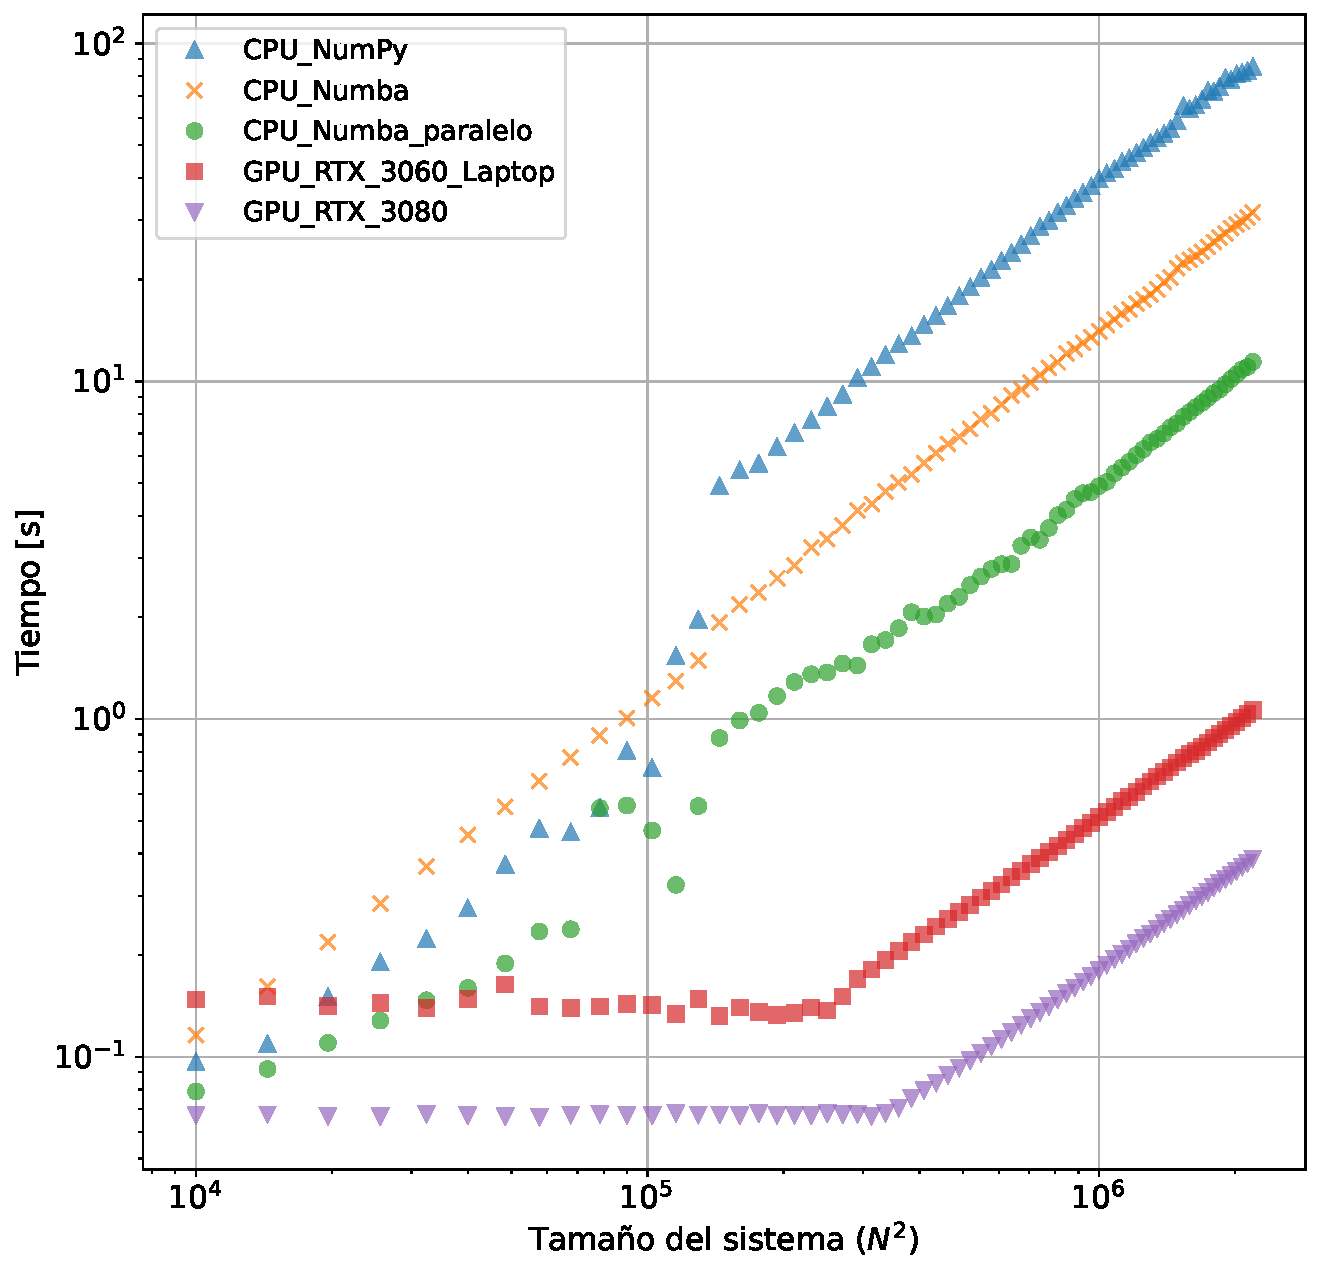
\includegraphics[width=\textwidth]{cpuvsgpu.pdf}
  \caption{}
\end{subfigure}
\begin{subfigure}{.6\textwidth}
  \centering
  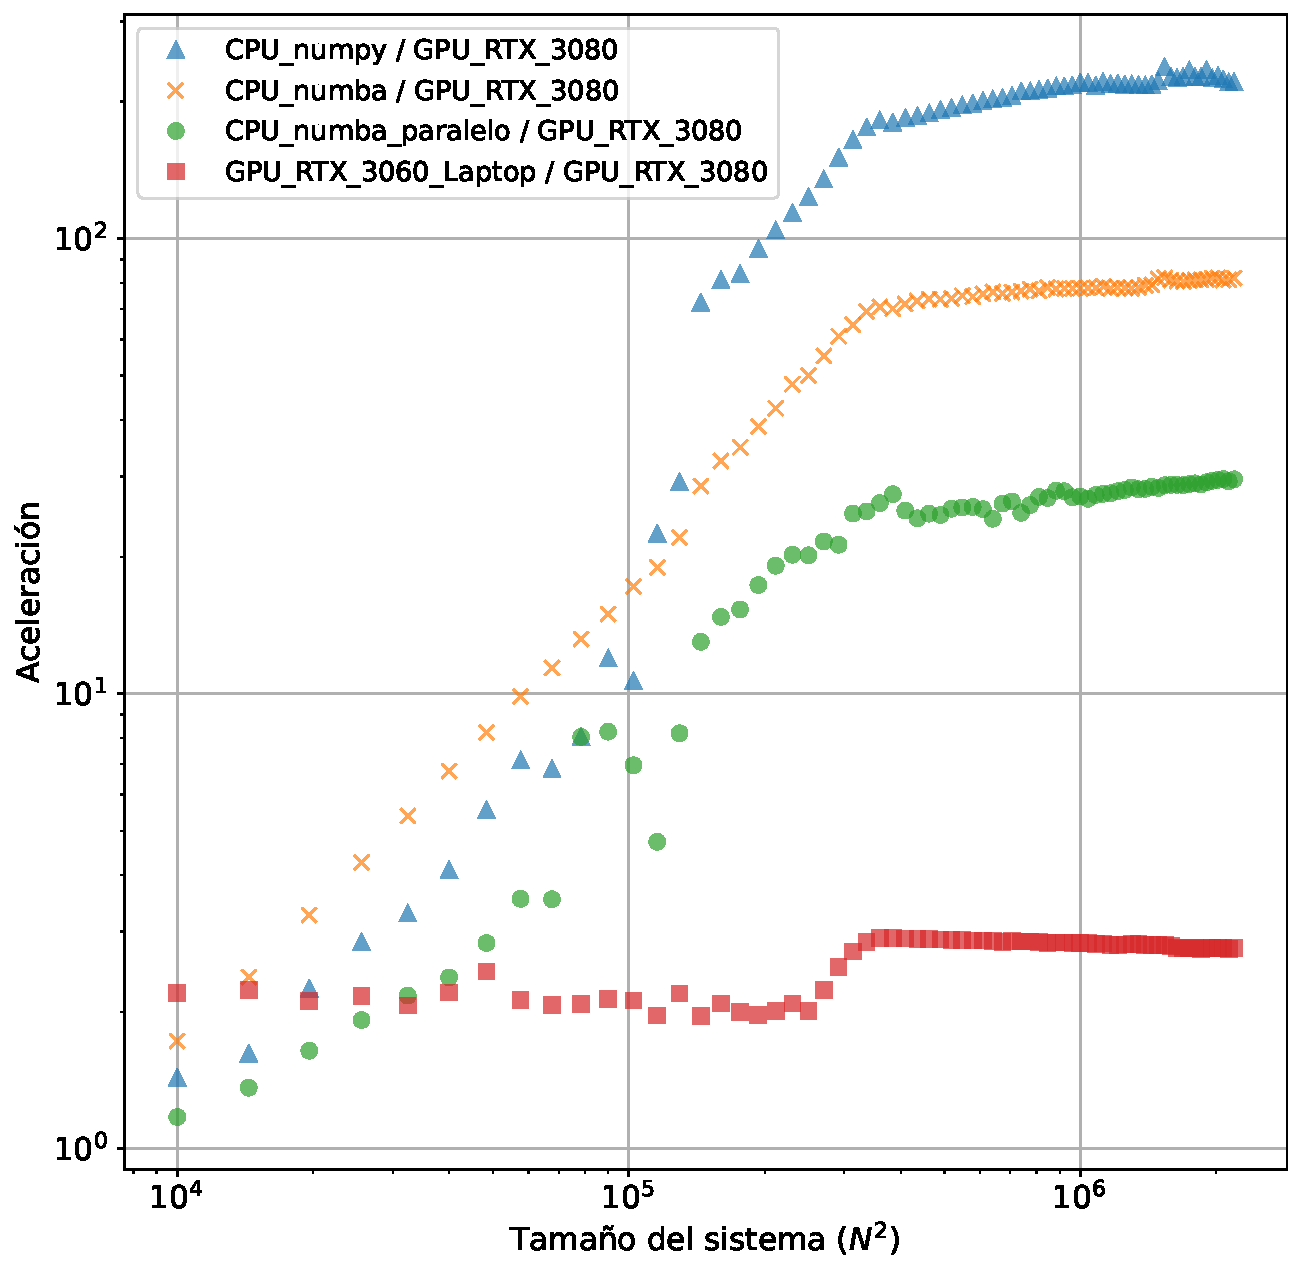
\includegraphics[width=\textwidth]{cpuvsgpu_ratio.pdf}
  \caption{}
\end{subfigure}
\caption{\textbf{(a)} Tiempo de simulación en función del tamaño del sistema $N \times N$ para las distintas implementaciones. \textbf{(b)} Aceleración 
obtenida al usar GPU en función del tamaño del sistema $N \times N$ para las distintas implementaciones.}
\label{fig:cpuvsgpu}
\end{figure}

Finalmente, es posible que quienes estén más interiorizados con \textit{CUDA} tal vez estén sorprendidos por el carácter superficial con el que 
usamos la GPU aquí. Es decir, cuando escribimos el \textit{kernel} no lo escribimos en \textit{CUDA C} o \textit{CUDA C++}, es algo similar, pero 
es distinto, lo cual puede confundir un poco. Además, en ningún momento indicamos cantidad de hilos por bloque ni cantidad de bloques en la grilla. 
Esto es, nuevamente, porque \textit{CuPy} intenta simplificar todo lo posible el uso de la GPU, para que sea accesible a usuarios sin conocimientos 
de \textit{CUDA}. Sin embargo, \textit{CuPy} ofrece también todo el acceso al detalle, tal como podría hacerse con \textit{CUDA C} por ejemplo,
y admite la escritura de \textit{kernels} directamente en \textit{CUDA C} a través de la función 
\href{https://docs.cupy.dev/en/stable/user_guide/kernel.html}{\textit{cupy.RawKernel}}. En el material complementario de este capítulo, dejo la 
implementación usando esta función que da acceso completo a \textit{CUDA}. No la agrego acá porque entiendo que no aporta demasiado, adicionalmente, no 
pude obtener ninguna mejora notable respecto al \textit{kernel} escrito con \textit{cupy.ElementwiseKernel}.











